\documentclass[12pt,a4paper,titlepage]{article}
%\documentclass[a4paper,twoside]{article} 
%\documentclass[12pt,a4paper,twoside]{article} 

\usepackage[pdftex]{graphicx}
%\usepackage[pdftex,draft]{graphicx}

\usepackage[latin1]{inputenc}
\usepackage[english]{babel}
\usepackage[pdftex,
	% remove to generate the printout version
	colorlinks=true,
	%citecolor=black,
	%urlcolor=black
	pdfauthor={Andreas Reufer},
	pdftitle={SPHLATCH  -- Parallelizing clumps, forests and families},
	pdfkeywords={tree, octree, parallel}
]{hyperref}

\usepackage{amssymb, amsmath}
\usepackage{mathrsfs}
\usepackage{amsfonts}

%\footnotesep0.5cm

\usepackage{aas_macros}

%\usepackage[T1]{fontenc}
%\usepackage{pxfonts}

%% One and a half spacing
\usepackage{setspace}

\usepackage{a4wide}
\usepackage{enumerate}

\usepackage{natbib}
\bibpunct{(}{)}{;}{a}{}{,}

\usepackage{verbatim}
\usepackage{moreverb}
\let\verbatiminclude\verbatimtabinput
\def\verbatimtabsize{4\relax}

\usepackage{algorithmic}
\usepackage{algorithm}

\newcommand{\ud}{\boldsymbol{d}}
\newcommand{\rvec}{\boldsymbol{r}}
\newcommand{\rsvec}{\boldsymbol{r'}}
\newcommand{\rivec}{\boldsymbol{r}_i}
\newcommand{\vvec}{\boldsymbol{v}}
\newcommand{\avec}{\boldsymbol{a}}
\newcommand{\xvec}{\boldsymbol{x}}
\newcommand{\Xvec}{\boldsymbol{X}}
\newcommand{\Qtens}{\boldsymbol{Q}}

\author{Andreas Reufer}
\title{SPHLATCH  -- Parallelizing clumps, forests and families}

\begin{document}
\pagestyle{headings}

\maketitle

\tableofcontents

%\begin{spacing}{1.5}

%% Sections
%% original problem

\section{A problem and one of its solutions}

\subsection{the N-Body problem}
One way of simulating a physical system is representing it with particles each carrying information about physical quantities. For example a system of $N$ gravitationally interacting bodies like stars in a galaxy, where the representation by particles is natural. When $\xvec_{i}$ is the position and $m_i$ the mass of particle $i$, then the acceleration of particle $j$ caused by gravitational interaction can be calculated by the \emph{direct sum}
\begin{equation}
\avec_j = - G \sum_{i \ne j} \frac{m_i}{r_{ij}^2} \frac{\rvec_{ij}}{r_{ij}} ~~~~ \text{where}~\rvec_{ij} = \rvec_j - \rvec_j
\end{equation}

So we have to evaluate $N$ sums with $N-1$ terms, a problem with complexity $O(N^2)$. By using Newtons third law the number of calculations can be reduced to half this number, but the order of complexity is still the same.\\

%short-range, long-range physics, inherent problem of n-body simulations

\subsection{The multipole approximation}
\label{multipoleapprox}
One solution to this problem is to use the multipole approximation. The idea is simple: Combine particles in spatial proximity into \emph{clusters}. When calculating the interactions of a single distant particle $j$ at $r_j$ with a cluster of particles $i$ at $r_i$  (where $j~\epsilon~C$) we can use as an approximation
\begin{align}
\avec_j &= - G \sum_{i~\epsilon~C} \frac{m_i}{r_{ij}^2} \frac{\rvec_{ij}}{r_{ij}} \approx - G \frac{m_{C}}{r_{Cj}} \frac{\rvec_{Cj}}{r_{Cj}} ~~~~ \text{when}~r_{ij} \gg r_{jk} ~~~ \forall j,k ~ \epsilon~C \\
m_C &= \sum_{i~\epsilon~C} m_i ~~~~ \rvec_C = \frac{1}{m_C} \sum_{i~\epsilon~C} \rvec_i m_i ~~~~ \rvec_{Cj} = \rvec_j - \rvec_C 
\end{align}

This is called the \emph{monopole approximation} and approximates the gravitational potential of the cluster of particles with a single gravitational monopole with mass $m_C$ at $\rvec_C$. This is a good approximation when the distance between the single particle and the cluster is big compared to the distances between the particles of the cluster between each other. The reason why the complexity of the computation gets lower, is that these two quantities are calculated once before the acceleration calculation and can be reused also for other distant particles. \\

This method can also be used with higher multipole moments which get arbitrarily complicated. We will now use the same denominations like in \cite{1993ApJ...414..200M}. The index $c$ stands for the particles constituting a clump, the \emph{children} of a clump. Indices $i, j, l$ number the three spatial dimensions. So the center of mass of a clump with children of masses $m_{c}$ and positions $\xvec_{c}$ can be written as
\begin{equation}
X_{i} = \frac{1}{M} \sum_{c} m_{c} x_{i, c} ~~~~~~~~ \text{for}~M > 0
\end{equation}

The total mass of the clump or in more technical terms, the rank-0 monopole tensor yields
\begin{equation}
M = \sum_{c} m_c \\
\end{equation}

the symmetric and traceless rank-2 quadrupole tensor, where $\rvec = \xvec_{c} - \Xvec $ denotes the position of the particle relative to the center of mass
\begin{equation}
Q_{ij} = \sum_{c} m_c \big( 3 r_{i, c} r_{j, c} - \rvec_{c}^2 \delta_{i j} \big) \\
\end{equation}

and the rank-3 octupole tensor which can be reduced to a rank-2 tensor
\begin{equation}
S_{ij}  = \sum_{c} m_c \big[ 5 \big( 3 - 2  \delta_{i j} \big) r_{i, c}^2 - 3 \rvec_{c}^2 \big] r_{j, c}\\
\end{equation}

and a rank-0 tensor component yield
\begin{equation}
S_{1 2 3} = 15 \sum_{k} m_c r_{1, c} r_{2, c} r_{3, c}
\end{equation}

Of cource the series continues with higher order multipole moments, but we will stop here as the approximation with multipoles moments up to the octupole is already pretty good for most cases. This representation of multiple particles as a clump with a center of mass and its multipole moments is a special case of the more general case, where the children of the parent cluster are also clusters with multipole moments. For the parent clump the monopole moment yields again

\begin{equation}
\label{eq_monopole}
M = \sum_{c} M_{c}
\end{equation}

the quadrupole tensor now includes the quadrupole moments of the children 
\begin{equation}
\label{eq_quadrupole}
Q_{ij} = \sum_{c} M_{c} \big( 3 r_{i, c} r_{j, c} - \rvec_{c}^{2} \delta_{i j} \big) + Q_{i j, c} 
\end{equation}

the octupole tensor components yields
\begin{align}
\label{eq_octupole}
S_{ij} = \sum_{c}&  M_{c} \big[ 5 \big( 3 - 2 \delta_{i,j} \big) r_{i, c}^{2} - 3 \rvec_{c}^2 \big] r_{j, c} 
+ 5 \big( 1 - \delta_{i j} \big) r_{i, c} Q_{i j, c} \nonumber \\
&+ \frac{5}{2} r_{j, c} Q_{i i, c} - \sum_{l} \big[ r_{l, c} Q_{j l, c} \big] + S_{i j, c} \\
S_{1 2 3} =& 15 \sum_{c} M_{c} r_{1, c} r_{2, c} r_{3, c} + \frac{5}{3} \big( r_{1, c} Q_{2 3, c} + r_{2, c} Q_{3 1, c} + r_{3, c} Q_{1 2, c} \big) + S_{1 2 3, c }
\end{align}

The center of mass is given again by
\begin{equation}
X_{i} = \frac{1}{M} \sum_{c} M_{c} X_{i, c} ~~~~~~~~  M > 0
\end{equation}

So particles can be treated like clusters with only a monopole moment and vanishing higher order multipoles.\\

The gravitational potential of a cluster can now be approximated in terms of its multipole moments up to the octupole
\begin{equation}
\phi(\rvec) = G \bigg(
\underbrace{ - \frac{M}{r} }_{monopole} ~ 
\underbrace{ - \frac{Q_{i j}}{r^{3}} \frac{r_{i} r_{j} }{2 r^{2} } }_{quadrupole}~ 
\underbrace{ - \frac{S_{i j}}{r^{4}} \frac{r_{i}^2 r_{j}}{2 r^{3} } + \frac{ S_{1 2 3} }{r^{4}}\frac{ r_{1} r_{2} r_{3} }{2 r^{3}} }_{octupole}~ 
+ O\Big(\frac{1}{r^{7}}\Big) \bigg)
\end{equation}

and so the acceleration for a point mass at $\rvec$ in this potential yields
\begin{align}
\label{eq:mpacc}
a_{k} &= - \nabla_{k} \phi(\rvec) \approx - G \bigg(
\underbrace{ \frac{M}{r^{2}} \frac{r_{k}}{r} }_{monopole}+ 
\underbrace{ \frac{Q_{i j}}{r^{4}}
\big( \frac{\delta_{i k} r_{j} }{r} + \frac{5 r_{i} r_{j} r_{k} }{2r^{3}} \big)
}_{quadrupole} \nonumber \\
&+ \underbrace{ \frac{S_{i j}}{r^{5}}
\big( \frac{ \delta_{i k} r_{i} r_{j} }{r^{2}}
+ \frac{ \delta_{j k} r_{i}^{2} }{2 r^{2} }
- \frac{7 r_{i}^{2} r_{j} r_{k} }{r^{4} } \big) 
 + \frac{S_{1 2 3}}{r^{5} }
\big( \frac{\delta_{1 k} r_{2} r_{3} + \delta_{2 k} r_{3} r_{1} + \delta_{3 k} r_{1} r_{2}}{2 r^{2}} 
- \frac{7 r_{1} r_{2} r_{3} r_{k} }{2 r^{4}}\big) 
}_{octupole}
\bigg)
\end{align}


%% a little excursion about trees

\section{the Barnes \& Hut tree algorithm}
In the previous chapter we saw a general formalism on how a cluster of particles can be approximated by multipole moments relative to their center of mass. This formalism however does not propose how to partition a given set of particles into clusters and clusters of clusters. The \emph{Barnes \& Hut tree algorithm} proposed in \cite{1986Natur.324..446B} does exactly that with the help a tree, a datastructure well suited to imply a hierarchy on a set of elements, in this case particles and clusters.

\subsection{A little excursion about trees}
First we need to know a few basic things about trees. A graph is a set of elements represented by \emph{nodes}. A tree is a rooted, directed graph in which any two nodes are connected by one and only one path. This means a node is the \emph{root node} and the connections between the nodes have a direction. Each node can have a number of children\footnote{often the term \emph{daughter} is used, but because of the asexual nature of tree nodes we are using here the term \emph{child}} 
nodes and has exactly one parent, expect for the root node which has no parent. Nodes can be assigned a depth. The root node per definition has depth $0$ and the children of a node have the inherit the depth of the parent increased by one. Figure \ref{fig:simpletree} shows a simple tree. The blue square represents the root node and has two children with depth 1, while on of this children has again two children with depth 2. Tree data structures are usually drawn upside-down, this means with the root on top and increasing depth to the bottom.

\begin{figure}[htbp]
\begin{center}
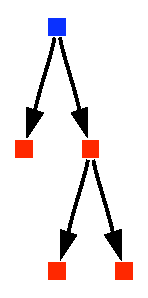
\includegraphics{simpletree.pdf}
\caption{A simple tree. the squares represent nodes which are interconnected by arrows pointing from the parent node to its children}
\label{fig:simpletree}
\end{center}
\end{figure}

Nodes without children are called \emph{leaf nodes}. A disjoint set of trees is called a \emph{forest}. One notices that the definition for a tree does not only fit the whole set of nodes of a tree, but also subsets. Every node can be taken as a root node and forms again a tree, also called a \emph{subtree} of the tree. Or one can say, that the children of a node form a forest of trees.

\subsection{Tree walks}
A tree walk is a sequence going through all the nodes of a tree once. For a tree with $N$ nodes there exist $N!$ possible tree walks, a few of them are special which are useful for the Barnes \& Hut tree algorithm.

\begin{figure}[htbp]
\begin{center}
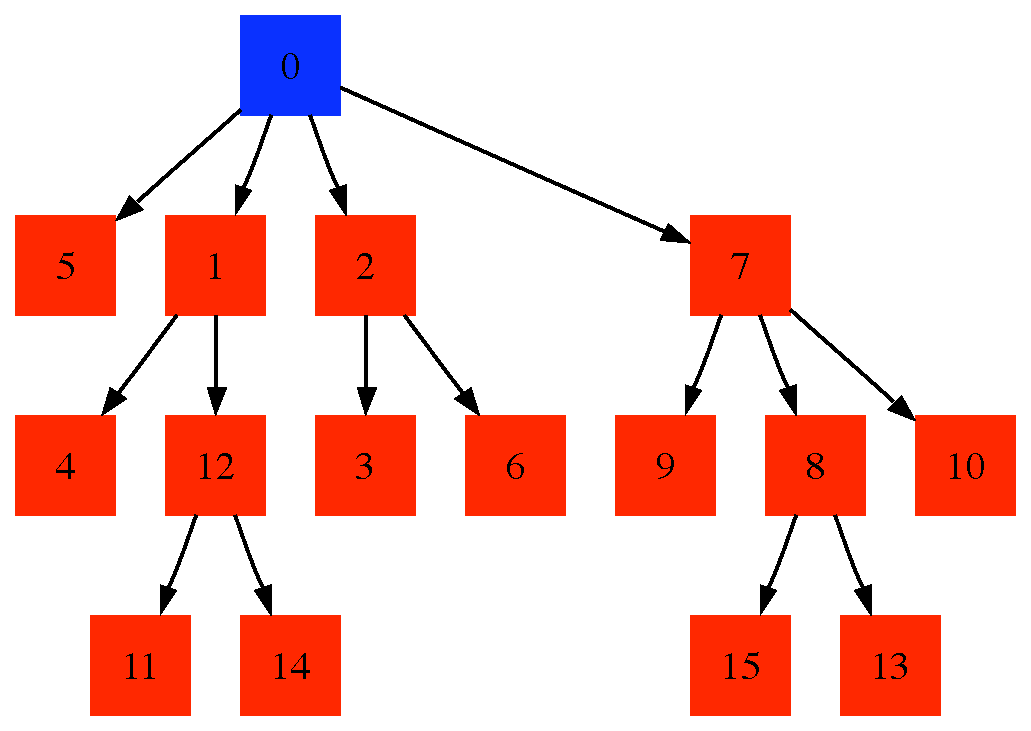
\includegraphics[scale=0.4]{simple_numbered_tree.pdf}
\caption{A slightly more complex tree with arbitrarly numbered nodes.}
\label{fig:simplenumtree}
\end{center}
\end{figure}

\paragraph{post order}
The post order tree walk starts at the root node. It can be implemented as shown in the following recursive algorithm
\begin{algorithm}
\caption{post order walk}
\begin{algorithmic}
\label{alg:postorder}
\STATE{pick current node}
\FORALL{children}
\STATE{go to child}
\STATE{do post order walk}
\ENDFOR
\end{algorithmic}
\end{algorithm}
\\

When $f_{post} (n)$ stands for applying the post order algorithm to node $n$ and the children are iterated from left to rigth, then the post order walk for the tree in figure \ref{fig:simplenumtree} can be elaborated in the following way
\begin{align}
\big\{& f_{post} (0) \big\} \nonumber \\
\big\{& 0, f_{post} (5),  f_{post} (1),  f_{post} (2),  f_{post} (7) \big\} \nonumber \\
\big\{& 0, 5, 1, f_{post} (4), f_{post} (12), 2, f_{post} (3), f_{post} (6), 7, f_{post} (9), f_{post} (8), f_{post} (10)\big\} \nonumber \\
\big\{& 0, 5, 1, 4, 12, f_{post} (11), f_{post} (14), 2, 3, 6, 7, 9, 8, f_{post} (15), f_{post} (13), 10 \big\} \nonumber \\
\big\{& 0, 5, 1, 4, 12, 11, 14, 2, 3, 6, 7, 9, 8, 15, 13, 10 \big\} \nonumber 
\end{align}

The key property of this walk is, that a node is not walked by unless every node on the path between the node and the root node has been walked. This property is useful, if a calculation on a node depends on results from the parent node.

\paragraph{pre order}
The pre order walk is similar to the post order walk, the only difference is that the children are walked before picking the current node. This gives the algorithm

\begin{algorithm}
\caption{pre order walk}
\begin{algorithmic}
\label{alg:preorder}
\FORALL{children}
\STATE{go to child}
\STATE{do pre order walk}
\ENDFOR
\STATE{pick current node}
\end{algorithmic}
\end{algorithm}

When $f_{post} (n)$ stands for applying the post order algorithm to node $n$, then the post order walk for the tree in figure \ref{fig:simplenumtree} can be elaborated in the following way

 %f_{post} ()
\begin{align}
\big\{& f_{pre} (0) \big\} \nonumber \\
\big\{& f_{pre} (5),  f_{pre} (1),  f_{pre} (2),  f_{pre} (7), 0\big\} \nonumber \\
\big\{& 5, f_{pre} (4), f_{pre} (12), 1,  f_{pre} (3),  f_{pre} (6), 2,  f_{pre} (9),  f_{pre} (8), f_{pre} (10), 7, 0\big\} \nonumber \\
\big\{& 5, 4,  f_{pre} (11),  f_{pre} (14), 12, 1, 3, 6, 2, 9,  f_{pre} (15),  f_{pre} (13), 8, 10, 7, 0\big\} \nonumber \\
\big\{& 5, 4, 11, 14, 12, 1, 3, 6, 2, 9, 15, 13, 8, 10, 7, 0\big\} \nonumber
\end{align}

The key property of the pre order walk, is that a node is not walked until all its children and their subtrees have been walked. Again, this is useful, if a calculation on a node depends on results from the children nodes.

\subsection{Trees for spatial subdivision}
A tree datastructure can be used to recursively subdivide space. The basic idea is to take a volume, assign this volume to a node in a tree, then subdivide this volume in disjoint subvolumes and assign these subvolumes to the children of the node. So the subdivision of space can be mapped onto a tree.\ The easiest form of subdivision is using volumes aligned with the dimensions and having the same side length in each dimension. So in 2D this corresponds to squares and in 3D to cubes along the axis. This volumes are then divided along each dimension into two equal-length intervals, which leads to $2^d$ subvolumes in $d$ dimensions. So if we have an arbitrary volume with a minimum $x_{i,min}$ and a maximum $x_{i,max}$ in each coordinate $i$ we can enclose this volume with a volume with sidelength $l$ and the center $x_{i,c}$

\begin{equation}
l = \max_{i} ( x_{i,max} - x_{i,min})  ~~~~ x_{i,center}= \frac{ x_{i,min} + x_{i,max} }{2}
\end{equation}

The $2^{d}$ subvolumes indexed with $j$ have a side length of $\frac{l}{2}$ and center vector components $i = 0 \dots d$, where $d_{i}$ stands for $i^{th}$ digit of the binary representation of the subvolume index $j$

\begin{equation}
x_{i, j~center} = x_{i,center} + l \frac{(-1)^{d_{i} + 1}}{2} ~~~~~ d_{i} = \frac{j  - \sum_{k \ne i} ( j \mod 2^{k} )}{2^{i}}
\end{equation}

In 2D this subvolumes are called \emph{quadrants}, in 3D \emph{octants}. The corresponding trees to which this subdivision can be mapped to are called \emph{quadtrees} and \emph{octrees}, having up to 4 and 8 children per node.

\subsection{the B\&H algorithm}
The Barnes \& Hut algorithm described in \cite{1986Natur.324..446B} subdivides the computational universe containing $N$ gravitationally interacting particles in subvolumes, called \emph{cells}. The particles are children of cell nodes. The tree must be built in a way, such that no cell octant contains more than one particle. An example of such a tree is shown in figure \ref{2D_CHtree} for 50 randomly distrbuted particles in 2D. 

\begin{figure}[htbp]
\begin{center}
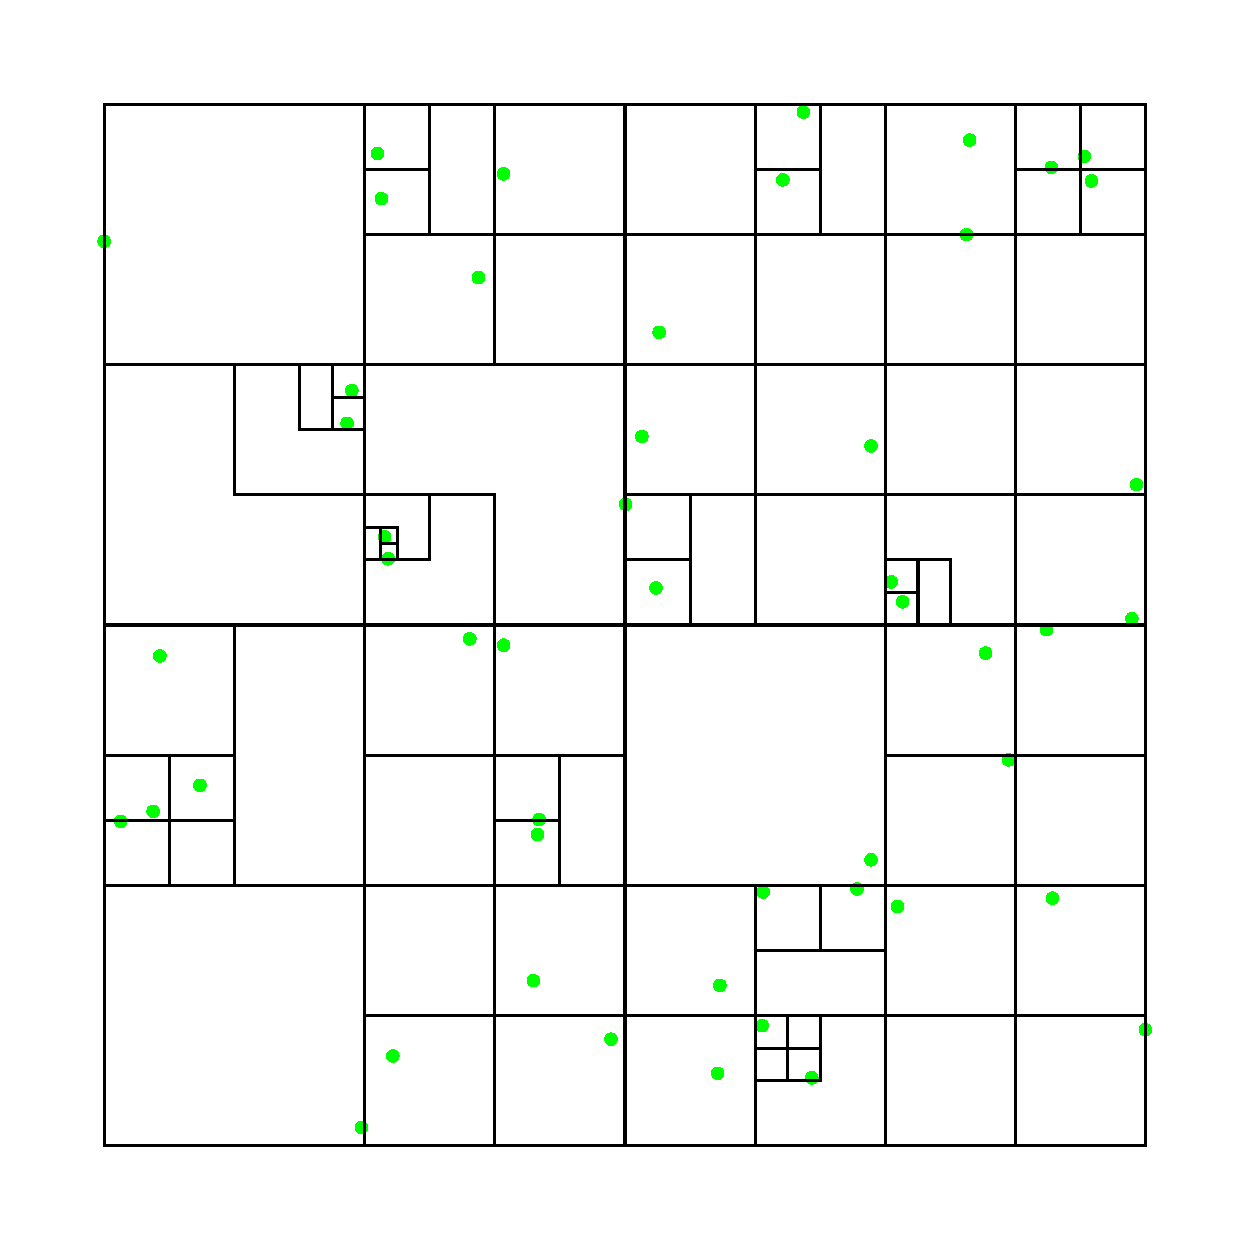
\includegraphics[scale=0.6]{quadtree50_xy.pdf}
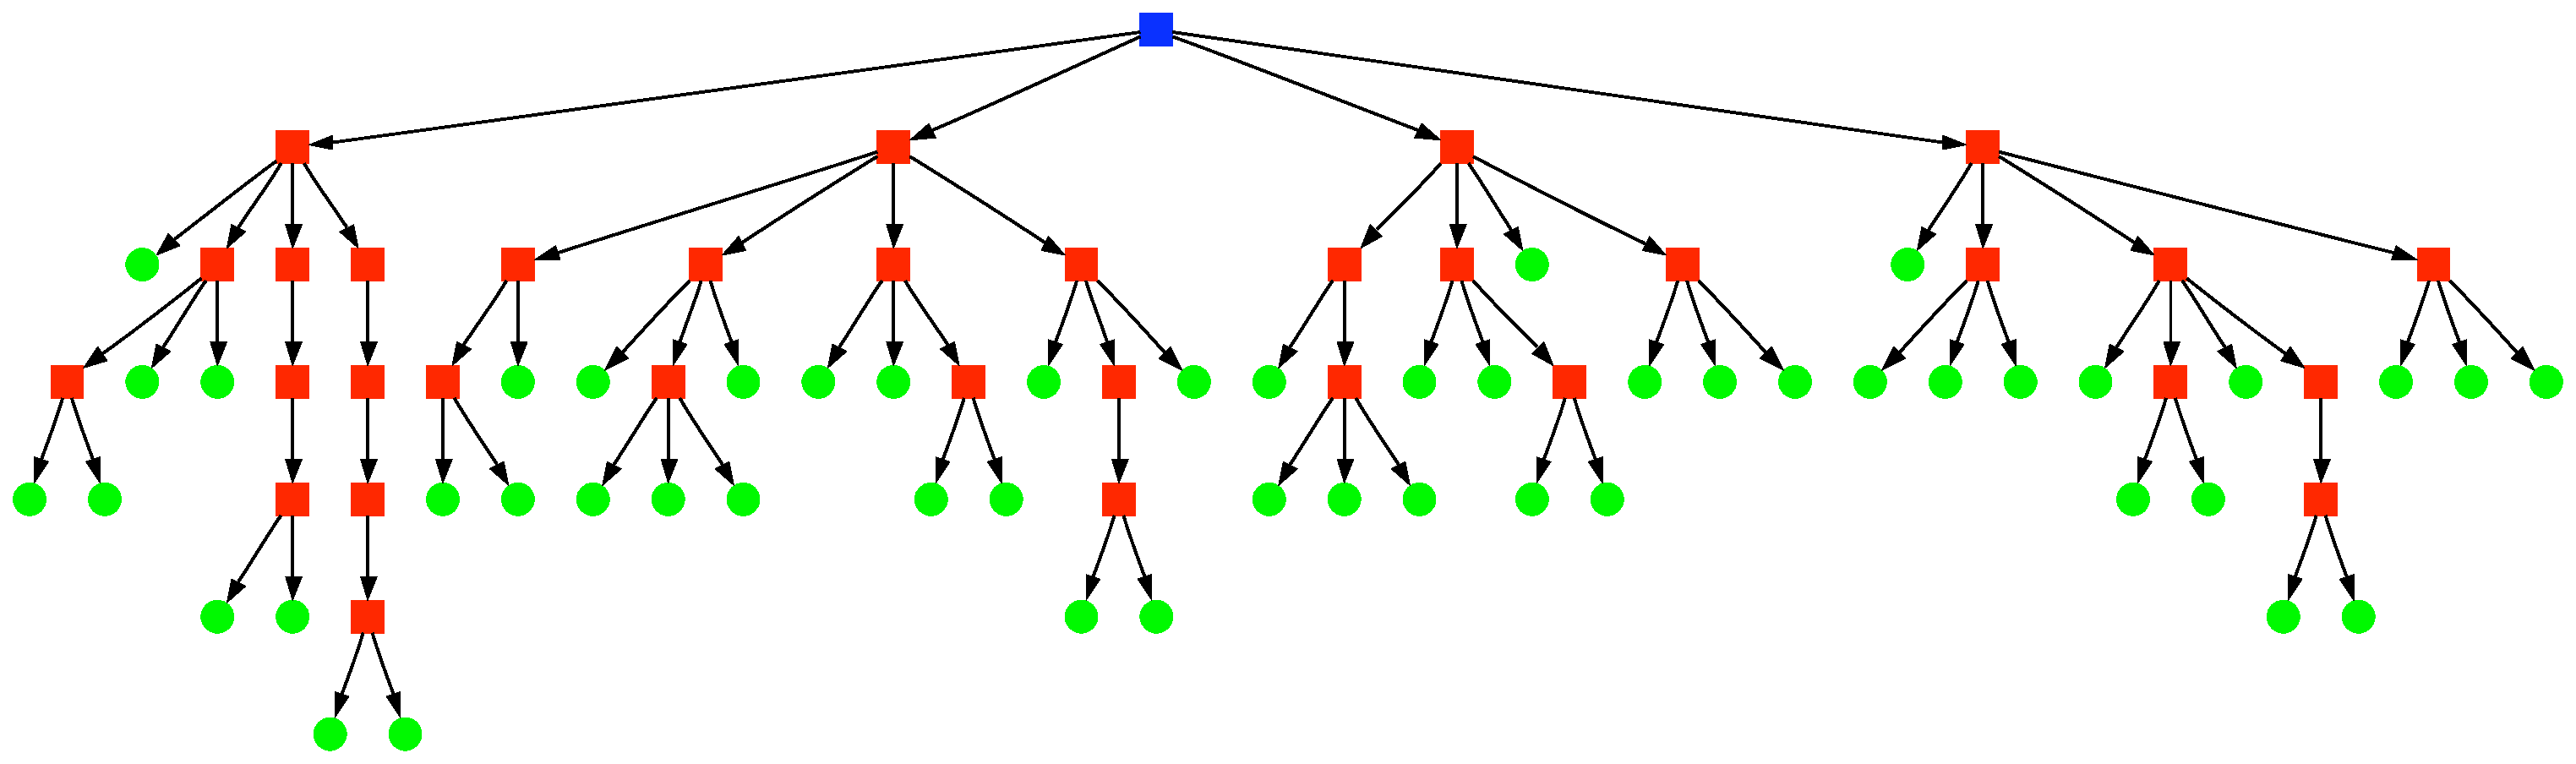
\includegraphics[scale=0.3]{quadtree50.pdf}
\caption{50 particles randomly distributed in $2D$ and the partitioning into cells (upper plot) with the and the corresponding \emph{quadtree} (lower plot)}
\label{fig:2D_BHtree}
\end{center}
\end{figure}



\begin{figure}[htbp]
\begin{center}

\includegraphics{ttnode_filled_local.pdf}

\includegraphics{ttnode_empty_local.pdf}

\includegraphics{node_filled_local.pdf}

\includegraphics{node_filled_remote.pdf}
\hspace{1cm}

\includegraphics{particle_filled_local.pdf}

\includegraphics{particle_filled_remote.pdf}
\caption{Symbols used for tree nodes. Squares stand for \emph{cells}, circles for \emph{particles}}
\label{fig:nodetypes}
\end{center}
\end{figure}


Each cell in the tree represents now a clump of particles. 

$\theta$ clumping parameter, self-acceleration for $\theta \ge 1$

%% implementation

\section{SPHLATCH - An implementation}

This section shows an approach to parallelize a Barnes \& Hut tree in an easy way. A few code examples are given in C/C++ and pseudocode.

\subsection{Parallelizing a particle calculation}
To speed up a particle calculation, it is desirable to be able to let it run in parallel on multiple processes on individual processors. There exist many different parallel setups, the one considered here consists of multiple processors with strictly local memory not directly accessible by the remote processors. Interprocessor communication is possible through an API like MPI.\\

The computational cost for calculating the derivatives like acceleration due to gravity or some SPH-sum in an SPH calculation, is typically of the same magnitude for every single particle. So a natural way of parallelizing such a calculation is to divide the set of particles used in the calculation into about equally sized subsets. Each subset is then assigned to a process. These subsets can be created by subdividing the space in which all particles lie into \emph{computational domains}, volumes containing the desired subset of particles. These volumes are called \emph{cost-zone volumes}. For the parallelization method used for the tree, it is necessary to build these computational domains out of volumes with a side length of $l / 2^{d_{cz}}$, where $l$ is the side length of the root node of the octree or in other words the side length of the smallest cube containing all the particles aligned with the coordinate system. $d_{cz}$ is the \emph{cost zone depth}.
\begin{figure}[htbp]
\begin{center}
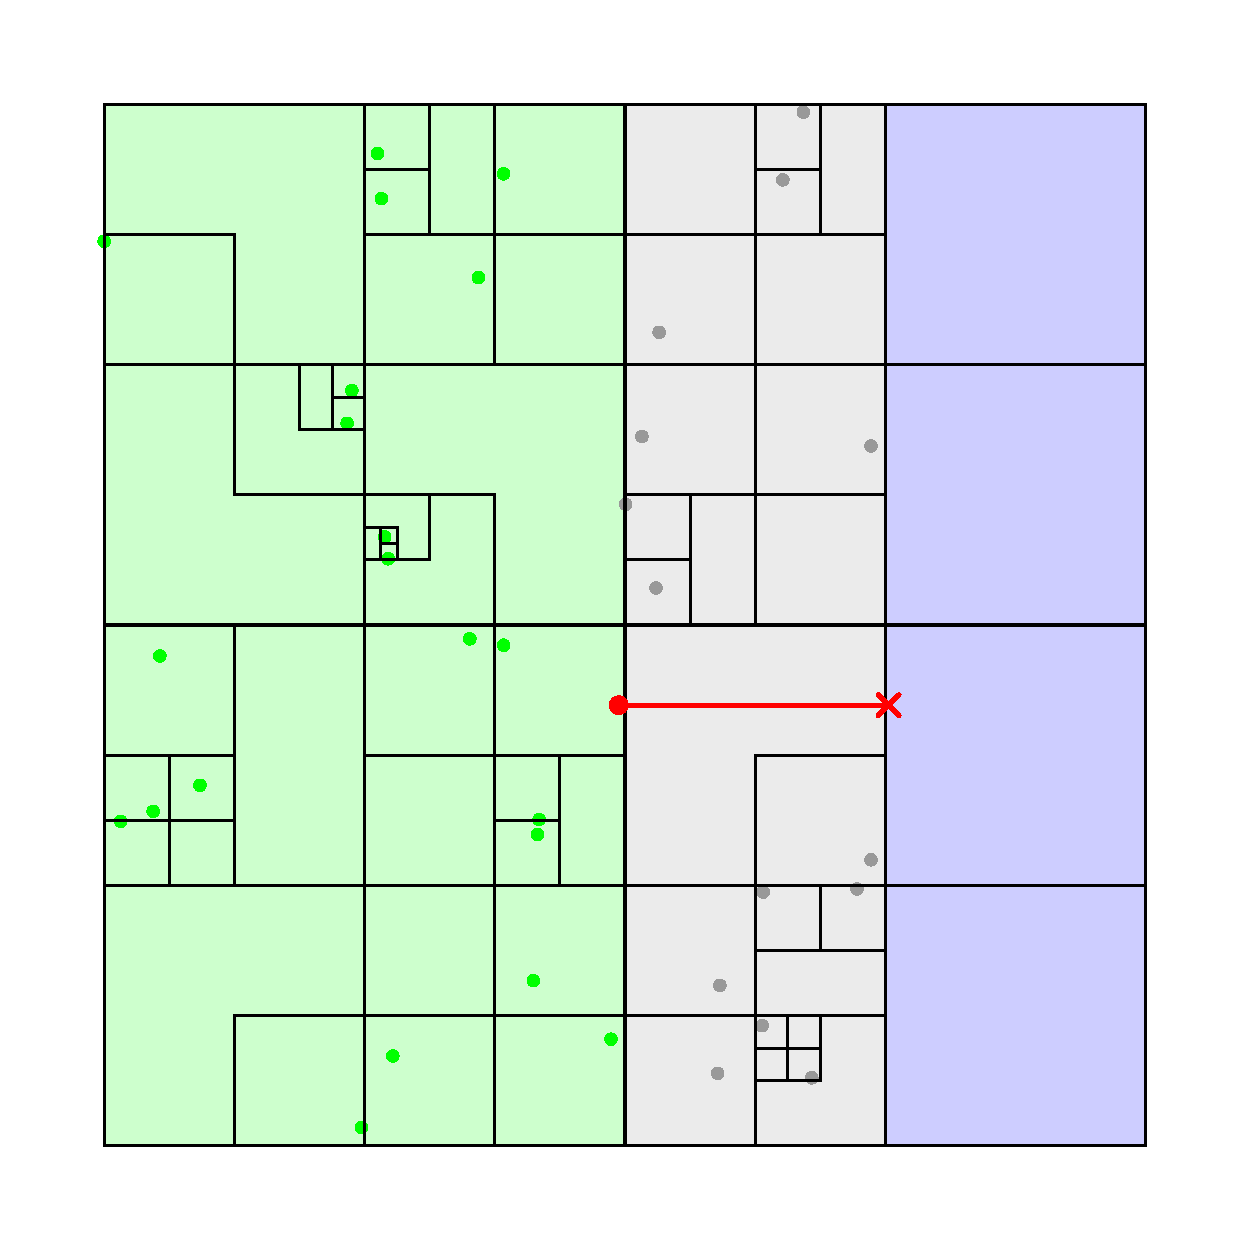
\includegraphics[scale=0.6]{quadtree50_xy_TPL2.pdf}
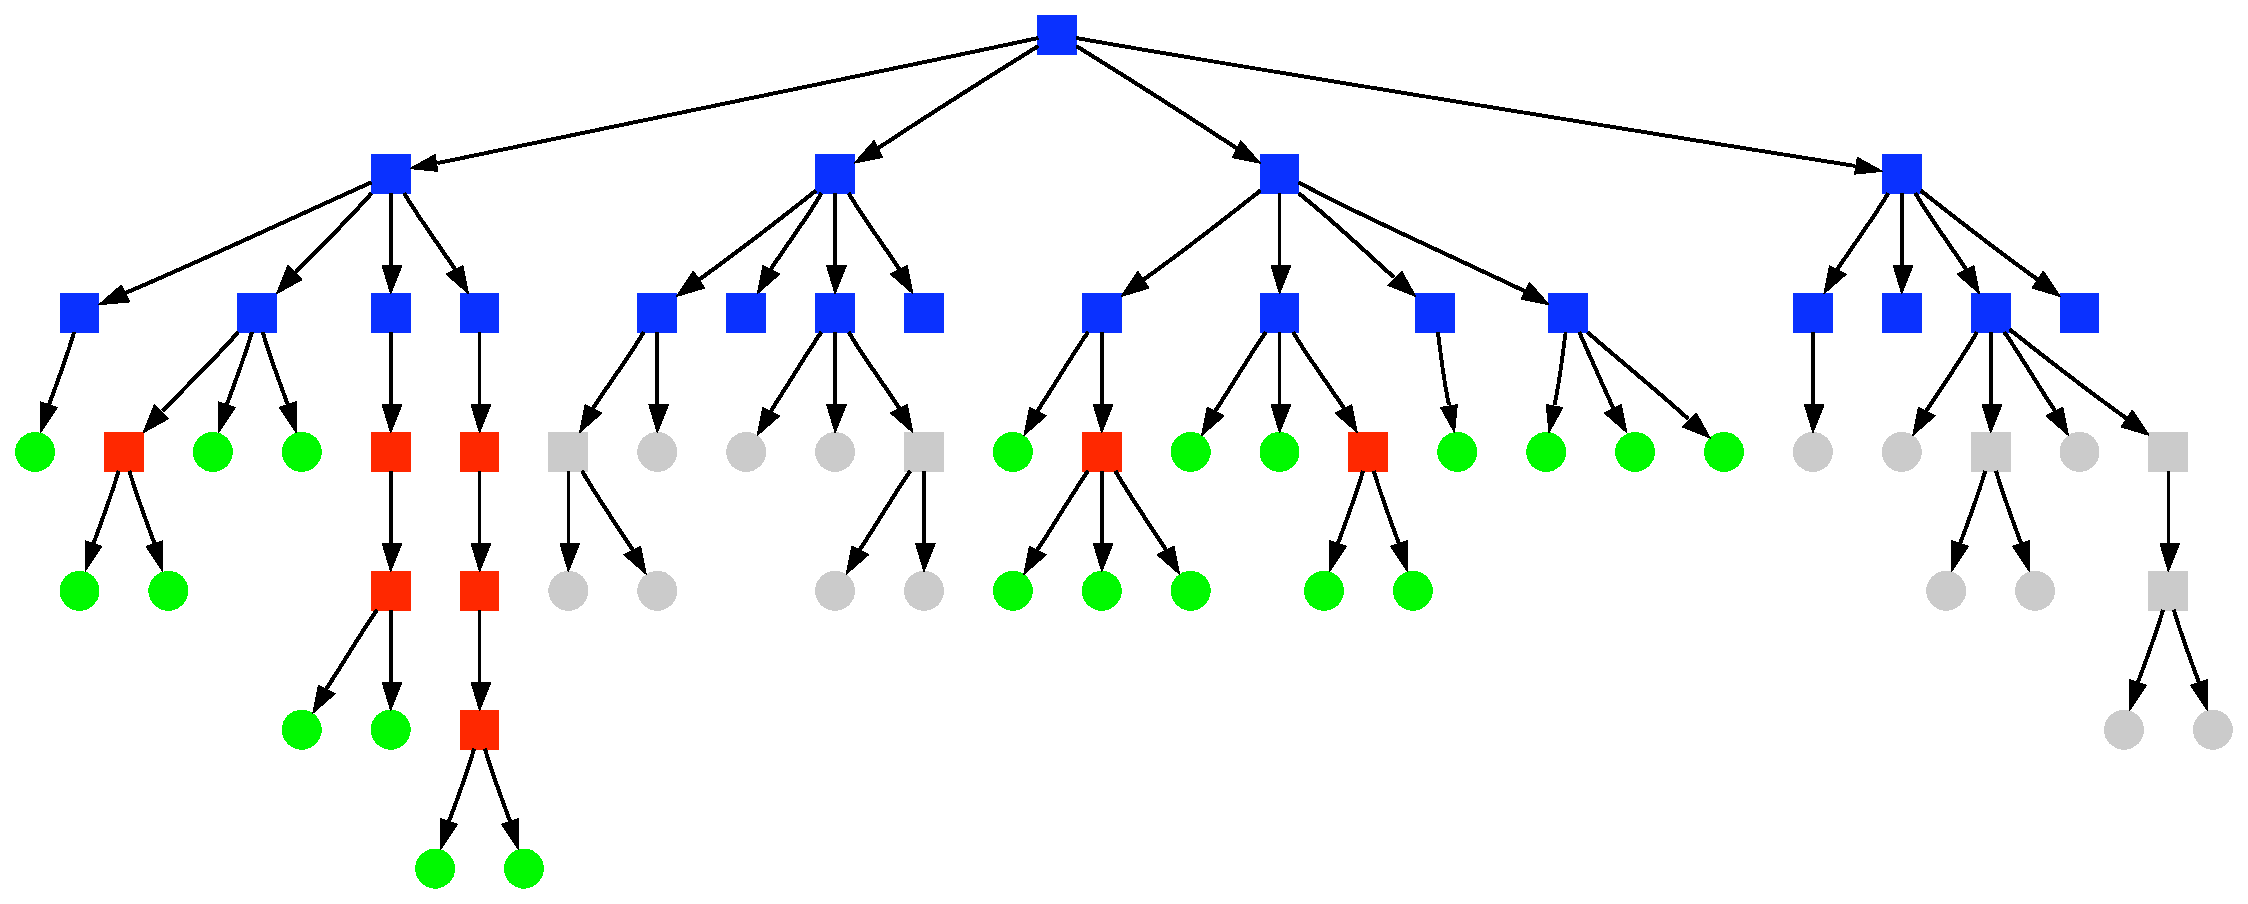
\includegraphics[scale=0.3]{quadtree50_TPL2_stage3.pdf}
\caption{A part of the same particle distribution like in figure \ref{fig:2D_BHtree}. The local domain is shaded green and contains 21 particles for which the acceleration has to be calculated. Bordering this zone is the ghost domain shaded grey, for which all particles are known. Beyond that, no particle information is available, only the corresponding parts of the global tree down to top-tree depth are known here. The plot below shows the corresponding tree. Note the filled top-tree nodes without any children nodes, they correspond to the domain where no particle information is available.}
\label{fig:2D_BHtree_costzone}
\end{center}
\end{figure}
Figure \ref{fig:2D_BHtree_costzone} shows one computational domain of such a partition of the same particle distribution like in figure \ref{fig:2D_BHtree}. The $21$ particles calculated in the current computational are called \emph{local particles} and are shown in green, the corresponding cost-zone volumes are shaded green. In this example the cost-zone depth is $2$ or the cost-zone volumes are obtained by subdividing space twice in each dimension. \\

Local particles may need information about particles in other computational domains. To compute an SPH-sum for a particle, usually information about particles within two smoothing lengths is needed. When a local particle is right at the edge of the domain, it needs to know about non-local particles in the adjacent domain. Particles inside non-local volumes sharing an edge with a local volume are called \emph{ghost particles} oder just \emph{ghosts}. Besided having to be copied on to the local process, they cause no computational cost, as only their information is used but nothing is calculated for them.\\

It is desirable to have as little ghost particles as possible. The way the computational domains and subsequently are made up by combining the cost-zone volumes determine the number of ghost. Generally it is best to minimize the surface of the computational domains. Composing the domains by cutting space-filling curves like the \emph{Peano-Hilbert-walk} along the cost-zone volumes into intervals leads usually to good results.\\

\subsection{Parallelizing a B\&H-tree}
Parallelizing the gravity calculation with a  B\&H-tree is not as straightforward like parallelizing a particle calculation for short-range forces, where interaction with distant non-local particles just can be omitted. The crucial point is to know, which parts the local particles need to know about the \emph{global tree} generated by all the particles, local and non-local. The tree known to the local particles is called the \emph{local tree} and provides all the necessary information to the local particles. It differs from the \emph{global tree} as such as it does not contain sub-trees not needed by the local particles. The sub-trees which can be omitted are be easily identified by the MAC and a worst-case scenario for the distribution of a local and a non-local particle shown in figure \ref{fig:2D_BHtree_costzone}. Assume a particle right at the edge of the computational domain, marked in the figure with a red dot. The shortest distance between this particle and any point in the non-local domain for which no particle information is available, marked in the figure with a red line, is the side length of the cost zone volumes or in other words the distance between the particle any point in the non-local domain $r_{WC}$ is always bigger than this side length:
\begin{equation}
r_{WC} \ge \frac{l}{2^{d_{CZ}} } 
\end{equation}
The MAC now tells us how big a cell might be to still be accepted for acceleration calculation, given the worst case distance or in other words, it tells us how deep we have to go in the tree until the multipole approximation is acceptable. Taking the worst case with distance $r_{WC}$ we get the deepest depth we have to go in the tree for a point in the non-local domain, we'll call that the \emph{top-tree depth} $d_{TT}$
\begin{equation}
\frac{l_{cell}}{r_{WC}} = \frac{l}{r_{WC} 2^{d_{TT}}} \ge \theta
\end{equation}
The top-tree depth is down to which the global tree has to be known on every computational domain. Any tree-structure below that depth is either provided by the local or ghost particles, or is not needed locally. Combining the two equations we get a relation between the top-tree depth, the costzone depth and the opening angle from the MAC:
\begin{equation}
2^{d_{CZ} - d_{TT}} \le \theta ~~~~\text{or}~~~~ d_{TT} = d_{CZ} + \uparrow \Big( - \frac{ \log{\theta} }{\log{2} } \Big)
\end{equation}
The first expression tells us down to which opening angle the local tree provides enough information for a given costzone and top tree depth. The latter expression gives the minimal needed top tree depth for a given costzone depth and opening angle. The rounding up is because depths are always integer numbers. The example shown in  figure \ref{fig:2D_BHtree_costzone} uses a top-tree depth of 2 and also a costzone depth of 2, so $\theta \ge 1$. In order to use a smaller opening angle we would have to increase the top-tree depth.\\

So we know now which parts of the global tree need to be in the local tree. The next question is how to build the local tree. On no process the global tree can be built, as no process knows about all the particles and also the global tree might be too big to fit into the memory available to a process. The basic idea is to build the local tree with local and ghost particles and then synchronize the \emph{top-tree} which is the global tree starting from the root node down to top-tree depth.
\begin{figure}[htbp]
\begin{center}
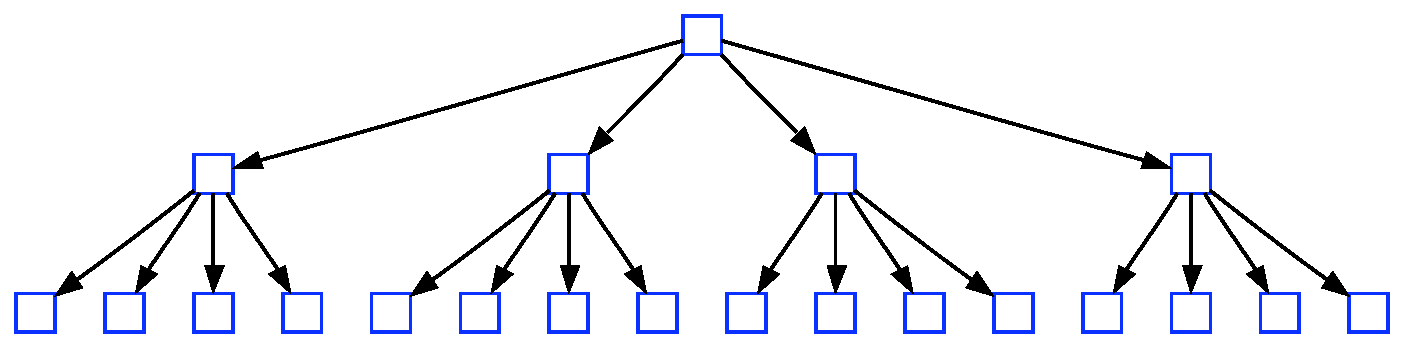
\includegraphics[scale=0.35]{quadtree50_TPL2_stage1.pdf}\\ \vspace{1.0cm}
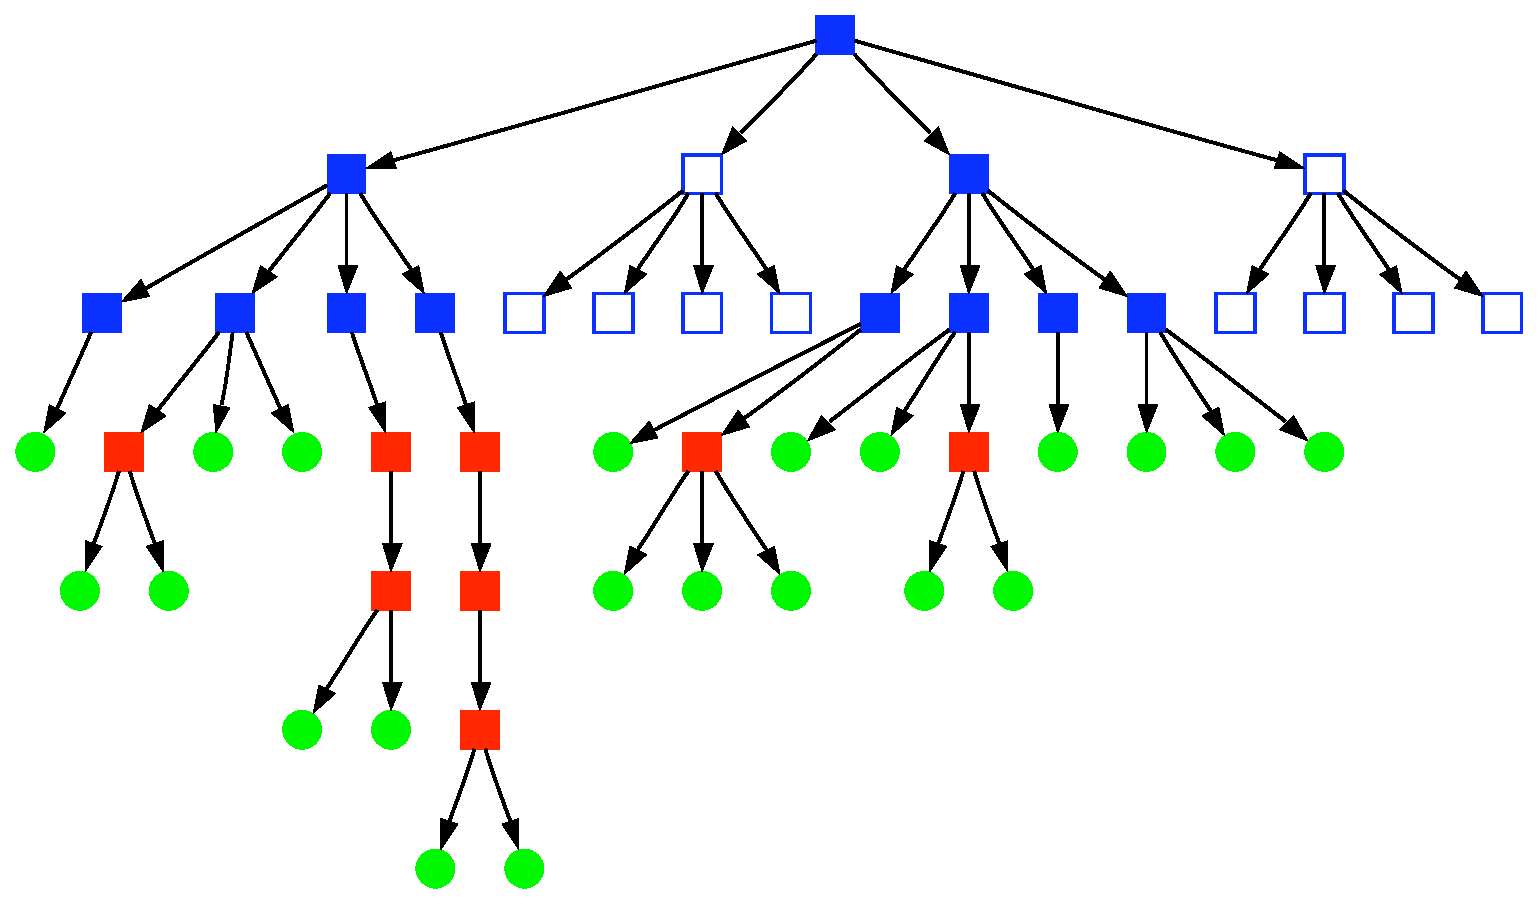
\includegraphics[scale=0.35]{quadtree50_TPL2_stage2a.pdf}\\
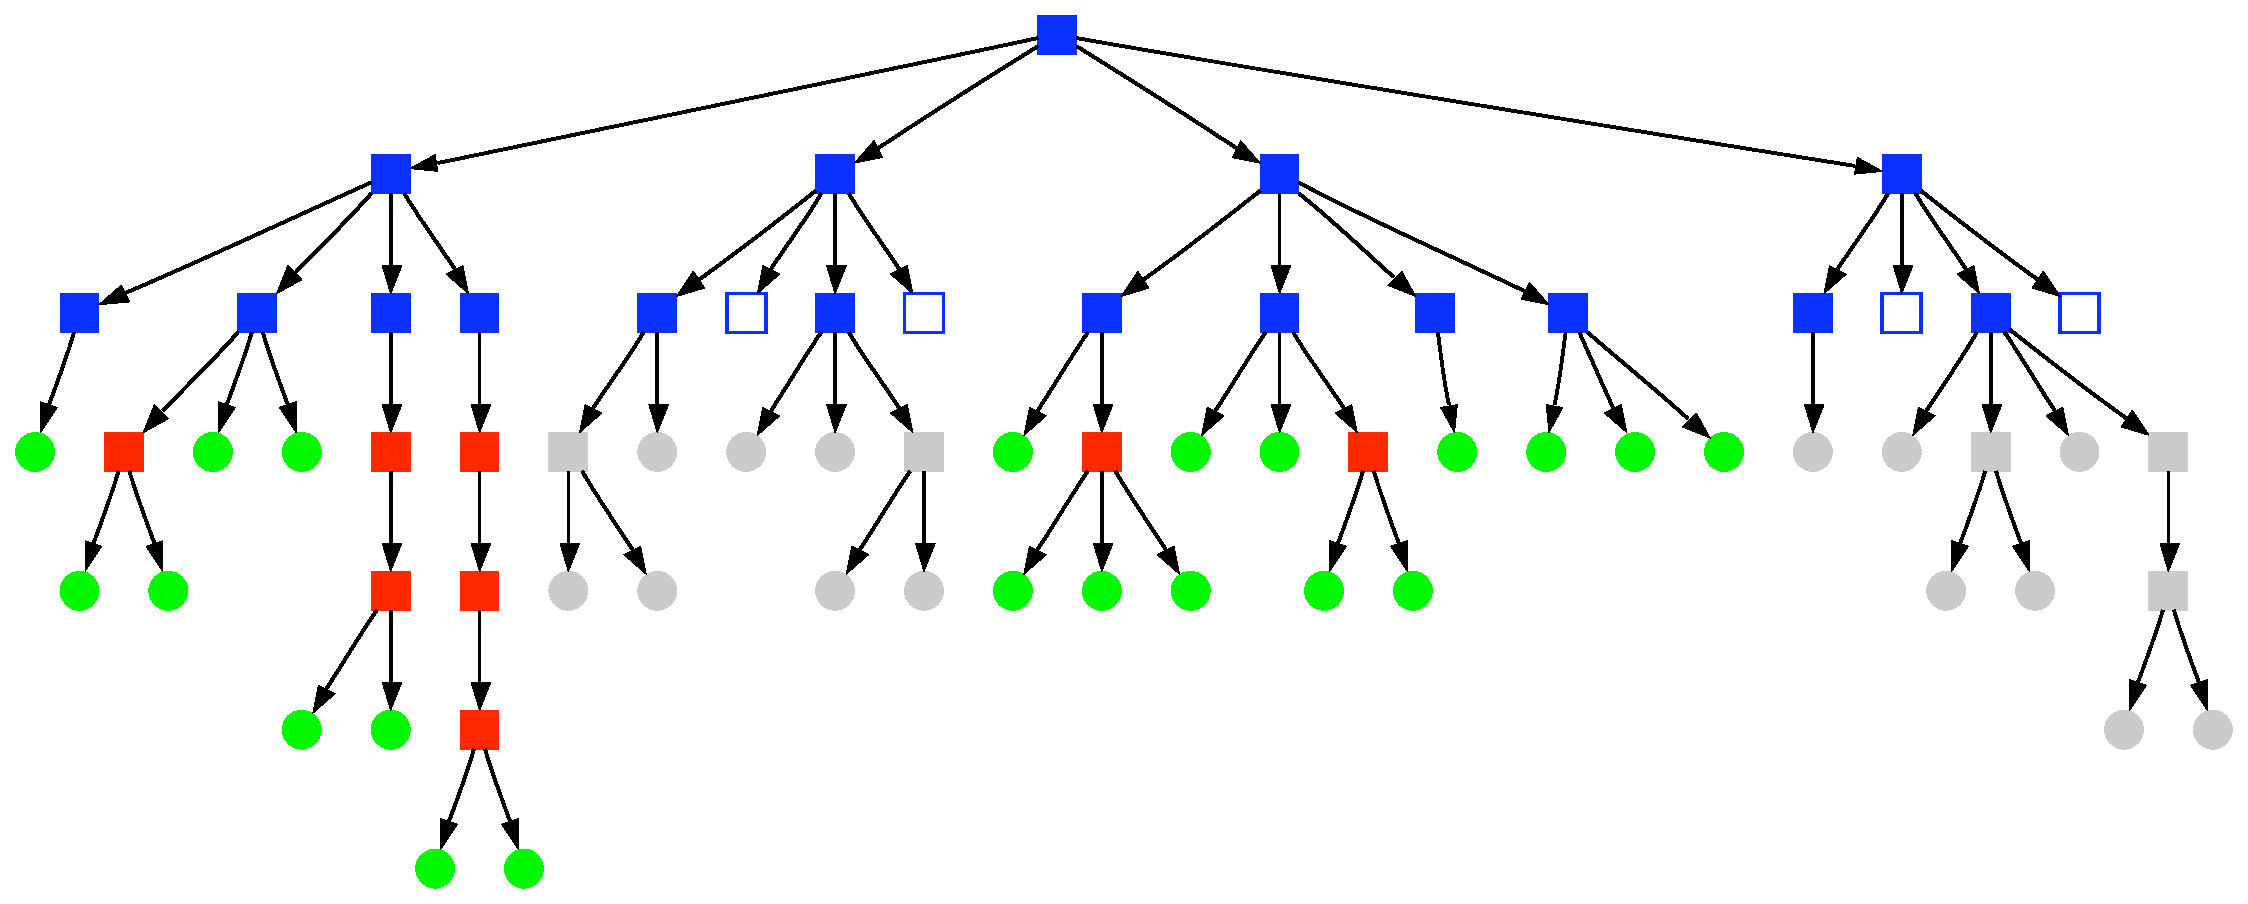
\includegraphics[scale=0.35]{quadtree50_TPL2_stage2b.pdf}\\
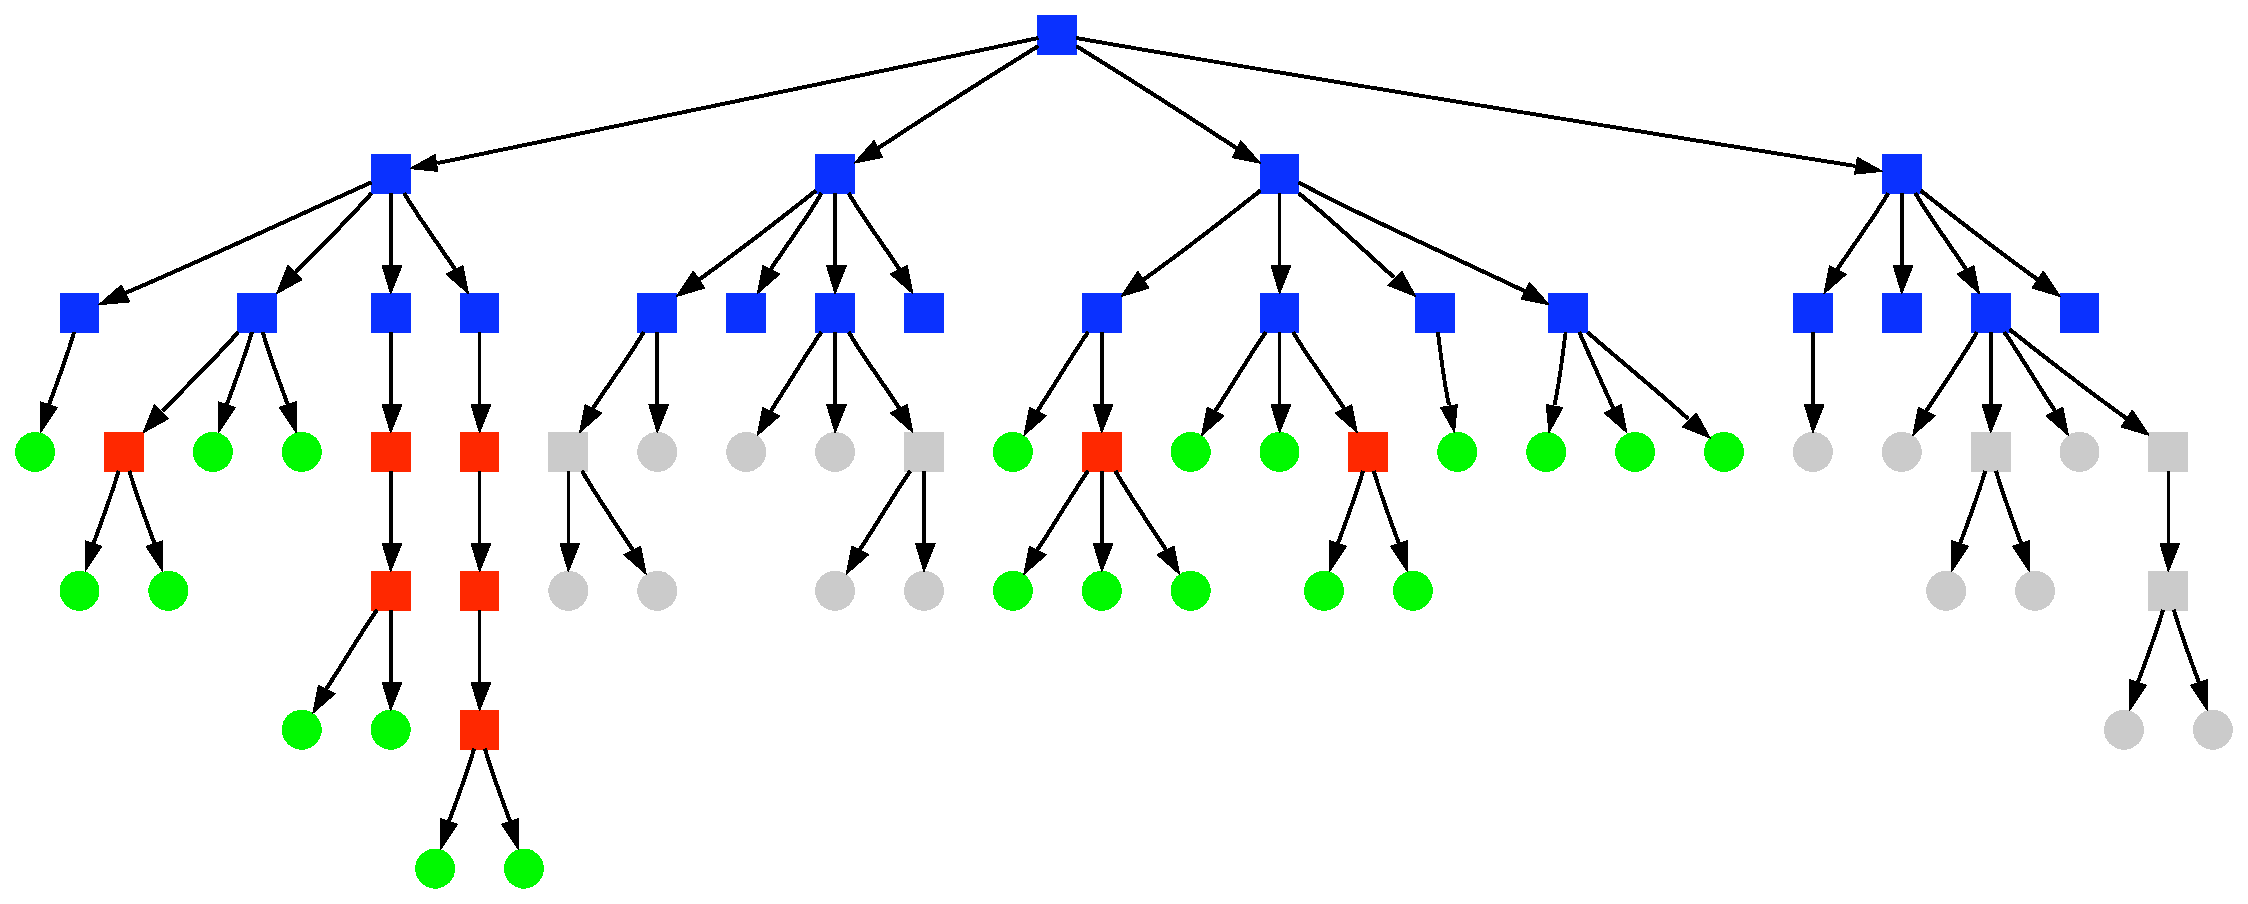
\includegraphics[scale=0.35]{quadtree50_TPL2_stage3.pdf}\\
\caption{Building stages of the local tree for the computational domain in figure \ref{fig:2D_BHtree_costzone}. The first tree shows the empty top-tree, a full quad-tree with depth 2. Then the local and the ghost particles are inserted leading to the second and third tree. As a final step the top-tree is summed up globally, filling up the 4 previously empty cell nodes. Top-tree cell nodes are coloured blue, normal cell nodes red and particles green. Ghost particles or cells are coloured grey. Non-filled shapes represent empty nodes.}
\label{fig:2D_BHtree_building}
\end{center}
\end{figure}\\

Synchronizing the top-tree is per se non-trivial, as a process does not know which parts of the non-local domain contain particles and therefore need nodes to represent them and which don't. The easiest solution is to build a \emph{full} top-tree, this means each node in the top-tree contains the maximum possible number of children. In 2D this corresponds to a full quad-tree, in 3D to a ful octree. The problem is now, that for non-uniform particle distributions we get many top-tree nodes not containing any particles in or below them, which will lead to unnecessary walks along them and vanishing contributions to the acceleration. The calculation does not get incorrect, but the adding up of vanishing terms leads to a higher computational cost. Therefore we introduce an \emph{emptiness} flag to each cell node. A priori a cell nodes is empty. Only when a particle is inserted the cell node becomes unempty or in other words filled. Emptiness is inherited bottom-up from the children to the parent node in a logically negative way, this means when a node has any non-empty child, it becomes non-empty. This flag can now be queried during tree-walks in order to avoid empty walking along empty sub-trees. So we start building the tree by setting up a full top-tree consisting of empty nodes. The first tree in figure \ref{fig:2D_BHtree_building} shows such an empty quadtree with top-tree depth of two. Every process now has a top-tree of the same structure and therefore we avoid synchronizing different tree structures between the processes.\\

During the next step, the particles locally known to a process, namely the local and ghost particles, are added to the local tree, inserting cell nodes where needed. After that the multipole moments can be calculated bottom-up from the children to their parents. This is a little bit tricky again, as a particle may be present on different process at the same time: On the process assigned to its computational domain as a local particle and to one or more domains as a ghost particle. We have to make sure, that such particles contribute to the multipole moments of the tree only once. But we also have to make sure, that the ghost particles contribute to the multipole moments of a ghost cell node. An example of such a ghost cell node can be seen in the third and fourth tree in figure \ref{fig:2D_BHtree_building} represented by grey squares. This ghost cell nodes may also be used for the acceleration calculation and therefore have to contain the correct multipole moments. For this reason we introduce a \emph{locality} flag to each node. A local particle has the locality \emph{local}, a ghost particle the locality \emph{remote}. Locality is again inherited bottom-up from the childred to their parent nodes in a positive sense. If one children is local, the parent node is also local. Only when all children are remote, the parent is remote. Top-tree nodes are excluded from this rule and have always the locality local. So when calculating the multipole moments of a node, we apply the rule that only nodes with the same locality contribute to the multipole moments. With that rule we fulfill both requirements mentioned above: Ghost cell and particle nodes do not contribute to the globally synchronized top-tree, but ghost cell nodes still get their correct multipole moments based on their remote or ghost children.\\

After adding up the multipoles, we can sum up the multipole moments of the top-tree. This is straightforward, as all top-trees have the same structure. The emptiness flag is summed up using an OR-relation, respecting the additive nature of multipole moments addition. After this step we end up with a valid Barnes\& Hut tree containing all the required particles and cells needed to calculate the gravitational acceleration for the local particles.\\

This parallelization method is rather simple, which is one of the advantages of it. Another advantage is, that after the particles and ghosts have been copied to the processes, only one, big additional communication step is required for summing up the multipole moments of the top-tree nodes. When summing up the multipole moments between two processes, all the data can be sent to one process and summed up there. This is bulk communication and therefore ideal for communication networks with high bandwidth. Latency is not important. In practice, the synchronization needs only a few percent of the total time of the gravity calculation using a reasonably fast network.\\

The downside of the method is that for non-uniform particle distribution a lot of unused and empty top-tree nodes have to be created. Although they don't need to be accessed, they use memory and worsen the caching of other tree nodes. The enforcement of cell nodes in the top-tree also causes a deeper tree than without the top-tree, which lead to longer and thereforce slightly slower tree walks.\\

\subsection{Implementing a tree datastructure}
The most common and probably also easiest way to implement a tree datastructure is by using \emph{pointers}. Pointers are a datatype pointing to another datatype, which can be a pointer again. One now defines a node datastructure, which is made up of pointers to others nodes, namely the parent node and the children node. If a child does not exist, corresponding pointer is set to the null pointer. As there may be more than one child, an array is used to store the child pointers with a size corresponding to the maximum number of children. Other information can also be stored in the tree node, for example in the case of a Barnes \& Hut tree the depth and the center coordinates of a cell.
\begin{verbatim}
struct node {
    node* parent;
    node* child[8];    // an octree
    int depth;
    
    // let's store some useful data on this node
    float centerX, centerY, centerZ;
    ...
}
\end{verbatim}

The tree can now be contructed by letting the nodes point to each other. If we don't want to have to access the tree nodes explicitely, it is necessary to define a \emph{cursor}. The cursor is a node pointer and can therefore point to any node in the tree. Data of the nodes can be accessed through the cursor. 
\begin{verbatim}
...
// assume we have the tree: Root -> Child0 -> Grandchild3
node* Cursor;
Cursor = *Root;               // initialize the Cursor
Cursor = Cursor->child[0];    // Cursor now points to Child0
Cursor->centerX = 42.;        // set centerX of Childo to 42
Cursor = Cursor->child[3];    // Cursor now points to Grandchild3
Cursor = Cursor->parent;      // ... to Child0 again
...
\end{verbatim}

Elementary tree operations can now be implemented, like going up to the parent node or going to a child.\\

Tree walks can be implemented be implemented by recursive functions, so called \emph{recursors}:
\begin{verbatim}
void postorderRecursor() {
    // do something
    useful();
    
    // walk existing children
    for (size_t i = 0; i < 8; i++) {        // assume 8 childs
         if ( Cursor->child[i] != NULL ) {  // does the child exist?
             goChild(i);
             postorderRecursor();           // recurse
             goParent();
         }
    }
}
...
goRoot();               // go to the root node
postorderRecursor();    // walk the tree
...
\end{verbatim}

The cursor will point to every tree node once in a post order and every time the function \verb|useful()| is executed. A pre-order tree walk or a walk of a subtree can be implemented in a similar fashion.\\

Each time the recursor calls itself, the current context is laid on to the stack, so the stack-depth is incremented by one. On a real-world computer, the stack has a finite size. When we want to walk a tree with mind-blowing depth, the stack depth will increase the deeper we go in the tree and will possibly overflow, leading to a program crash. So is recursion dangerous for tree walks? In the case of Barnes \& Hut trees it is not.\\

This can be shown with a quick back of a napkin calculation: Let's imagine a worst-case scenario with two particles positioned at almost the same coordinates. When trying to insert the second particle at almost the same place like the first particle, the two come to lie in the same cell octant so that a new children cell has to be created at this octant. Each time this happens, the resolution to distinguish the two particles increase by two or in other words, the the difference in coordinates of the particles has to be half as small in order for the tree not to be able to distinguish the two particles again. Or we can also say, one more bit of the binary representation of the particles coordinates have to match each other. Particle coordinates are usually stored as floating point numbers. A floating point number is usually represented according to the \emph{IEEE 754} standard, with 24 bits precision for a single precision float and 53 bits for a double precision float. So in a worst case, the tree gets a depth of around 24 or 53, a depth which can be handled by the stacks of modern computers. And yet this worst-case is very pathological, as a calculation with such high dynamics easily leads to other problems like over- or underflows. Concluding we can say, that recursion for the B\&H-tree walks is not dangerous.

\subsection{Implementing the B\&H-tree algorithm}
The gravitational acceleration calculation with a parallelized B\&H-tree like shown before breaks down to 4 major steps: Building the top-tree, inserting the particles and ghosts, calculating the multipole moments and finally calculating the resulting acceleration on the particles. If the tree is not needed any more, the tree has also to be deleted. For this five steps, there exist easy recursive algorithms.\\

After the root node has been created, the cursor is set to point to it. After that the top-tree is built by calling the top-tree build recursor.
%top-tree build algorithm
\begin{algorithm}
\caption{top-tree build recursor}
\begin{algorithmic}
\label{alg:buildtoptree}
\IF{ depth $\le$  top-tree depth}
\STATE{make emtpy cell node}
\FORALL{children}
\STATE{go to child}
\STATE{call top-tree build recursor}
\STATE{go to parent}
\ENDFOR
\ENDIF
\end{algorithmic}
\end{algorithm}

Inserting a particle into the tree can also be done with a recursive function. The idea is to start at the root node and try to insert the particle as a child of the current node. There are three cases possible: The child node does not exist, so the particle can be inserted directly. If there is already a cell node, go there and call the insertion function again. If there is already a particle node, save this particle temporarily and call the insertion function for this particle and the one that has been to be inserted in the first place. At the beginning of the recursor, the current node is set to be non-empty, so that the inserting a particle leaves a path from the root node to the particle of non-empty nodes.
%particle insertion algorithm
\begin{algorithm}
\caption{insert particle $p_{i}$ recursor}
\begin{algorithmic}
\label{alg:insertparticle}
\STATE{$k =$ subVolumeIndex($p_{i}$)}
\STATE{set current node to non-empty}
\IF{child $k$ is not existing }
\STATE{go to child $k$}
\STATE{make particle node, fill it with $p_{i}$}
\STATE{go to parent}
\ELSIF{child $k$ is a cell node}
\STATE{go to child $k$}
\STATE{call insert particle $p_{i}$ recursor}
\STATE{go to parent}
\ELSIF{child $k$ is a particle node}
\STATE{save particle from child $k$ to $p_{j}$}
\STATE{go to child $k$}
\STATE{convert particle node to cell node}
\STATE{call insert particle recursor for $p_{i}$}
\STATE{call insert particle recursor for $p_{j}$}
\STATE{go to parent}
\ENDIF
\end{algorithmic}
\end{algorithm}\\

When the tree has been built, the multipole moments can be calculated by iterating through all non-empty tree nodes in a pre-order fashion, so that the multipole moments of the children of a node are already calculated when the multipoles of the node has to be calculated. The multipoles calculation recursor starts at the root node. After its execution, all cell nodes below the top-tree contain the correct multipole moments, this is also the case for cell nodes containing ghost nodes. After executing the recursor, the multipoles in the top-tree are added up globally, so that also the top-tree cell nodes contain the correct multipole moments. This is done by summing up between processes pair-wise with a binary tree, so that even for a high number of processes there are not too many communication steps. The total of the multipoles is then distributed again to every process with the same binary in the opposite direction.
%multipole calculation algorithm
\begin{algorithm}
\caption{multipoles calculation recursor}
\begin{algorithmic}
\label{alg:multipolecalc}
\IF{current node is not empty }
\FORALL{existing children}
\STATE{go to child}
\STATE{call multipoles calculation recursor}
\STATE{go to parent}
\IF{ depth $>$ top-tree depth }
\STATE{determine locality of current node}
\STATE{calculate multipoles from children nodes with the same locality}
\ELSE
\STATE{calculate multipoles from local children nodes}
\ENDIF
\ENDFOR
\ENDIF
\end{algorithmic}
\end{algorithm}
\\

To calculate the acceleration due to gravity for a particle, a recursive tree walk starting from the root node has to be undertaken. The recursion is stopped, when either the MAC is fulfilled or the current node is a particle or empty. In order not to calculate the gravitational interaction of the particle with itself, before calling the algorithm, the particle node is made to look like an empty cell node, so that no interaction is calculated. After the execution of the algorithm, the corresponding node is changed back again to a particle node. The node of a particle can be directly accessed by following a node pointer saved for each particle in the tree. 
%acceleration algorithm
\begin{algorithm}
\caption{acceleration calculation recursor}
\begin{algorithmic}
\label{alg:calcgravity}
\IF{current node is a particle node}
\STATE{calculate acceleration due to a particle}
\ELSIF{current node is empty}
\STATE{do nothing}
\ELSIF{MAC is fulfilled}
\STATE{calculate acceleration due to a cell}
\ELSE
\FORALL{existing children}
\STATE{go to child}
\STATE{call acceleration calculation recursor}
\STATE{go to parent}
\ENDFOR
\ENDIF
\end{algorithmic}
\end{algorithm}\\

The tree has to be deleted again after the calculation. In order not to disconnect any nodes from the tree, the nodes are deleted in a pre-order fashion with algorithm \ref{alg:treedeletion}.
%tree deletion algorihm
\begin{algorithm}
\caption{tree deletion recursor}
\begin{algorithmic}
\label{alg:treedeletion}
\FORALL{existing children}
\STATE{go to child}
\STATE{call tree deletion recursor}
\STATE{go to parent}
\STATE{delete current node}
\ENDFOR
\end{algorithmic}
\end{algorithm}


% Include a bibliography
\bibliographystyle{plain}
%\bibliographystyle{natbib}
%\bibliographystyle{natdin}
%\bibliographystyle{abbrvnat}
%\bibliographystyle{unsrtnat}
%\bibliographystyle{plainnat}

\bibliography{bibliography}

% Appendix
\appendix
\section{Appendix}

\subsection{Explicit scalar expressions for adding up multipoles}

In practice we need scalar expressions for the multipole tensors and break up the sums given in equations \ref{eq_monopole} $-$ \ref{eq_octupole}. Given an existing parent clump with a center of mass $X'_{i}$ and multipole moments $M', Q'_{i j}, S'_{i j}, S'_{123}$ and another clump with $x_i, m, q_{i j}, s_{i j}, s_{123}$ we want to merge to the parent clump, we would like to be able to write the new multipole moments of the new parent cluster as
\begin{align}
M &= M' + \Delta M \nonumber \\
Q_{ij} &= Q'_{ij} + \Delta Q_{ij} \nonumber \\
S_{ij} &= S'_{ij} + \Delta S_{ij} \nonumber \\
S_{123} &= S'_{123} + \Delta Q_{123} \nonumber
\end{align}

The new center of mass can be calculated with
\begin{equation}
%X_{1} = X'_{1} \frac{M'}{M'+m} + x_1 \frac{m}{M'+m} ~~~~ X_{2} = X'_{2} \frac{M'}{M'+m} + x_2  \frac{m}{M'+m} ~~~~ X_{3} = X'_{3} \frac{M'}{M'+m} + x_3  \frac{m}{M'+m}
X_{1} = \frac{1}{M'+m} (X'_{1} M' + x_1 m) ~~~~ X_{2} = \frac{1}{M'+m} (X'_{2} M' + x_2 m) ~~~~ X_{3} = \frac{1}{M'+m} (X'_{3} M' + x_3 m) \nonumber
\end{equation}

The $\Delta$-expressions yield
\begin{align*}
\Delta M &= m \\
\Delta Q_{11} &= m (3 r_1^2 - \rvec^2) + q_{11} \nonumber \\
\Delta Q_{22} &= m (3 r_2^2 - \rvec^2) + q_{22} \nonumber \\
\Delta Q_{33} &= m (3 r_3^2 - \rvec^2) + q_{33} \nonumber \\
\Delta Q_{12} &= \Delta Q_{21} = m ( 3 r_1 r_2 ) + q_{12} \nonumber \\
\Delta Q_{13} &= \Delta Q_{31} = m ( 3 r_1 r_3 ) + q_{13} \nonumber \\
\Delta Q_{23} &= \Delta Q_{32} = m ( 3 r_2 r_3 ) + q_{23} \nonumber \\
\Delta S_{11} &= m ( 5 r_1^2 - 3 \rvec^2 ) r_1 + q_{11} (3/2) r_1 - q_{12} r_2 - q_{13} r_3 + s_{11} \nonumber \\
\Delta S_{22} &= m ( 5 r_2^2 - 3 \rvec^2 ) r_2 + q_{22} (3/2) r_2 - q_{12} r_1 - q_{23} r_3 + s_{22} \nonumber \\
\Delta S_{33} &= m ( 5 r_3^2 - 3 \rvec^2 ) r_3 + q_{33} (3/2) r_3 - q_{13} r_1 - q_{23} r_2 + s_{33} \nonumber \\
\Delta S_{12} &= m ( 15 r_1^2 - 3 \rvec^2 ) r_2 + q_{12} ( 4 r_1 + (5/2) r_2) - q_{22} r_2 - q_{23} r_3 + s_{12} \\
\Delta S_{21} &= m ( 15 r_2^2 - 3 \rvec^2 ) r_1 + q_{21} ( 4 r_2 + (5/2) r_1) - q_{11} r_1 - q_{13} r_3 + s_{21} \\
\Delta S_{13} &= m ( 15 r_1^2 - 3 \rvec^2 ) r_3 + q_{13} ( 4 r_1 + (5/2) r_3) - q_{23} r_2 - q_{33} r_3 + s_{13} \\
\Delta S_{31} &= m ( 15 r_3^2 - 3 \rvec^2 ) r_1 + q_{31} ( 4 r_3 + (5/2) r_1) - q_{11} r_1 - q_{12} r_2 + s_{31} \\
\Delta S_{23} &= m ( 15 r_2^2 - 3 \rvec^2 ) r_3 + q_{23} ( 4 r_2 + (5/2) r_3) - q_{13} r_1 - q_{33} r_3 + s_{23} \\
\Delta S_{32} &= m ( 15 r_3^2 - 3 \rvec^2 ) r_2 + q_{32} ( 4 r_3 + (5/2) r_2) - q_{12} r_1 - q_{22} r_2 + s_{32} \\
\Delta S_{123} &=15 \big( m r_1 r_2 r_3 + (5 / 3) ( q_{12}  r_3 + q_{13} r_2 + q_{23} r_1) + s_{123} \big)
\end{align*}

where $r_i = x_i - X_i$

\subsection{Preprocessing directives}
\verb| SPHLATCH_SINGLEPREC | \\
\verb| SPHLATCH_TREE_PROFILE |\\
\verb| SPHLATCH_MPI |\\



%\end{spacing}

\end{document}
